\documentclass[14pt]{book}
\usepackage[a4paper,
left=20mm,
top=25mm]{geometry}
\usepackage{fontspec}
\usepackage{xcolor}
\usepackage{polyglossia}
\newfontfamily\kannadafont{Noto Sans Kannada}
\setmainlanguage{kannada}
\setotherlanguages{english}

\usepackage{xcolor}
\usepackage{emptypage}
\usepackage{array}
\usepackage{multirow}
\usepackage{lastpage}
\usepackage{verbatim}
\usepackage[nomessages]{fp}
\usepackage{calc}
\usepackage{xstring}
\usepackage[alpine]{ifsym}
\usepackage{ifthen}
\usepackage{multido}
\usepackage{xargs}
\usepackage{tikz}
\usepackage{pgf}
\usetikzlibrary{calc, fadings, shadows.blur}
\usepackage{amsfonts,amsmath,amssymb,mathrsfs,amsthm}
\usepackage{lmodern}
\usepackage{multicol}
\usepackage[font={color=gray},skip=1pt, size=large]{caption}
\usepackage{ScratchX}

\linespread{1.7}
\begin{document}
\fontsize{13pt}{17pt}\selectfont
\begin{titlepage} % Suppresses headers and footers on the title page
	
	\centering % Centre everything on the title page
	
	%------------------------------------------------
	%	Top rules
	%------------------------------------------------
	
	\rule{\textwidth}{1pt} % Thick horizontal rule
	
	\vspace{2pt}\vspace{-\baselineskip} % Whitespace between rules
	
	\rule{\textwidth}{0.4pt} % Thin horizontal rule
	
	\vspace{0.1\textheight} % Whitespace between the top rules and title
	
	%------------------------------------------------
	%	Title
	%------------------------------------------------
\begin{center}	
	\textcolor{red}{ % Red font color
		{\Huge\textbf{ಕನ್ನಡದಲ್ಲಿ ಸ್ಕ್ರಾಚ್ ಪ್ರೋಗ್ರಾಮ್ಮಿಂಗ್\\ಭಾಗ - ೧}
	}
}
\end{center}
	\vspace{0.025\textheight} % Whitespace between the title and short horizontal rule
	
	\rule{0.3\textwidth}{0.4pt} % Short horizontal rule under the title
	
	\vspace{0.1\textheight} % Whitespace between the thin horizontal rule and the author name
	
	%------------------------------------------------
	%	Author
	%------------------------------------------------
	\begin{center}
	{\Large \textsc{ಡಾ\hspace{0.3mm}\vline\hspace{0.5mm}\vline \hspace{1mm}ಯು. ಬಿ. ಪವನಜ}}\\
	ಮತ್ತು\\
	{\Large \textsc{ಡಾ\hspace{0.3mm}\vline\hspace{0.5mm}\vline \hspace{1mm}ಆನಂದ್ ಸಾವಂತ್}} % Author name
	\end{center}
	
	\vspace{3cm} % Whitespace between the author name and publisher
	
\includegraphics[scale=0.4]{KKali_logo.pdf}
	\hspace{2cm}
	
\includegraphics[scale=0.19]{VishvaKannadaLogo.pdf}
%	\hspace{2cm}
%	
\includegraphics[scale=0.4]{KKali_logo.pdf}
	\vfill
	%------------------------------------------------
	%	Publisher
	%------------------------------------------------
	
	%{\large\textcolor{red}{\plogo}}\\[0.5\baselineskip] % Publisher logo
	
	{\large\textsc{ಪಬ್ಲಿಶರ್}} % Publisher
	
	\vspace{0.1\textheight} % Whitespace under the publisher text
	
	%------------------------------------------------
	%	Bottom rules
	%------------------------------------------------
	
	\rule{\textwidth}{0.4pt} % Thin horizontal rule
\begin{small}
\color{gray}{(ಸೂಚನೆ: ಈ ಟ್ಯುಟೋರಿಯಲ್‌ ಪುಸ್ತಕಕ್ಕೆ ಬಳಸಿದ್ದು ಸ್ಕ್ರಾಚ್ 1.4 ಆವೃತ್ತಿ)}\par
\end{small}

	\vspace{8pt}\vspace{-\baselineskip} % Whitespace between rules
	
	\rule{\textwidth}{1pt} % Thick horizontal rule
	
\end{titlepage}

\begin{center}
\Large\textbf{\color{blue}{ಮುನ್ನುಡಿ}}
\end{center}
\vspace{1cm}
ಮುನ್ನುಡಿ ಕೃತಿಯ ಲೇಖಕನಿಂದ ಬರೆಯಲಾದ ಒಂದು ಪುಸ್ತಕ ಅಥವಾ ಇತರ ಸಾಹಿತ್ಯ ಕೃತಿಗೆ ಪೀಠಿಕೆ. ಒಬ್ಬ ಬೇರೆ ವ್ಯಕ್ತಿಯು ಬರೆದ ಪರಿಚಯಾತ್ಮಕ ಪ್ರಬಂಧಕ್ಕೆ ಪ್ರಸ್ತಾವನೆ ಎಂದು ಕರೆಯಲಾಗುತ್ತದೆ ಮತ್ತು ಇದು ಲೇಖಕನ ಮುನ್ನುಡಿಗಿಂತ ಮೊದಲು ಬರುತ್ತದೆ. ಮುನ್ನುಡಿಯು ಹಲವುವೇಳೆ ಆ ಸಾಹಿತ್ಯ ಕೃತಿಯಲ್ಲಿ ನೆರವಾದವರಿಗೆ ವಂದನೆಗಳೊಂದಿಗೆ ಅಂತ್ಯಗೊಳ್ಳುತ್ತದೆ.ಮುನ್ನುಡಿ ಕೃತಿಯ ಲೇಖಕನಿಂದ ಬರೆಯಲಾದ ಒಂದು ಪುಸ್ತಕ ಅಥವಾ ಇತರ ಸಾಹಿತ್ಯ ಕೃತಿಗೆ ಪೀಠಿಕೆ. ಒಬ್ಬ ಬೇರೆ ವ್ಯಕ್ತಿಯು ಬರೆದ ಪರಿಚಯಾತ್ಮಕ ಪ್ರಬಂಧಕ್ಕೆ ಪ್ರಸ್ತಾವನೆ ಎಂದು ಕರೆಯಲಾಗುತ್ತದೆ ಮತ್ತು ಇದು ಲೇಖಕನ ಮುನ್ನುಡಿಗಿಂತ ಮೊದಲು ಬರುತ್ತದೆ. ಮುನ್ನುಡಿಯು ಹಲವುವೇಳೆ ಆ ಸಾಹಿತ್ಯ ಕೃತಿಯಲ್ಲಿ ನೆರವಾದವರಿಗೆ ವಂದನೆಗಳೊಂದಿಗೆ ಅಂತ್ಯಗೊಳ್ಳುತ್ತದೆ.
\vspace{1cm}

ಮುನ್ನುಡಿ ಕೃತಿಯ ಲೇಖಕನಿಂದ ಬರೆಯಲಾದ ಒಂದು ಪುಸ್ತಕ ಅಥವಾ ಇತರ ಸಾಹಿತ್ಯ ಕೃತಿಗೆ ಪೀಠಿಕೆ. ಒಬ್ಬ ಬೇರೆ ವ್ಯಕ್ತಿಯು ಬರೆದ ಪರಿಚಯಾತ್ಮಕ ಪ್ರಬಂಧಕ್ಕೆ ಪ್ರಸ್ತಾವನೆ ಎಂದು ಕರೆಯಲಾಗುತ್ತದೆ ಮತ್ತು ಇದು ಲೇಖಕನ ಮುನ್ನುಡಿಗಿಂತ ಮೊದಲು ಬರುತ್ತದೆ. ಮುನ್ನುಡಿಯು ಹಲವುವೇಳೆ ಆ ಸಾಹಿತ್ಯ ಕೃತಿಯಲ್ಲಿ ನೆರವಾದವರಿಗೆ ವಂದನೆಗಳೊಂದಿಗೆ ಅಂತ್ಯಗೊಳ್ಳುತ್ತದೆ.ಮುನ್ನುಡಿ ಕೃತಿಯ ಲೇಖಕನಿಂದ ಬರೆಯಲಾದ ಒಂದು ಪುಸ್ತಕ ಅಥವಾ ಇತರ ಸಾಹಿತ್ಯ ಕೃತಿಗೆ ಪೀಠಿಕೆ. ಒಬ್ಬ ಬೇರೆ ವ್ಯಕ್ತಿಯು ಬರೆದ ಪರಿಚಯಾತ್ಮಕ ಪ್ರಬಂಧಕ್ಕೆ ಪ್ರಸ್ತಾವನೆ ಎಂದು ಕರೆಯಲಾಗುತ್ತದೆ ಮತ್ತು ಇದು ಲೇಖಕನ ಮುನ್ನುಡಿಗಿಂತ ಮೊದಲು ಬರುತ್ತದೆ. ಮುನ್ನುಡಿಯು ಹಲವುವೇಳೆ ಆ ಸಾಹಿತ್ಯ ಕೃತಿಯಲ್ಲಿ ನೆರವಾದವರಿಗೆ ವಂದನೆಗಳೊಂದಿಗೆ ಅಂತ್ಯಗೊಳ್ಳುತ್ತದೆ.ಮುನ್ನುಡಿ ಕೃತಿಯ ಲೇಖಕನಿಂದ ಬರೆಯಲಾದ ಒಂದು ಪುಸ್ತಕ ಅಥವಾ ಇತರ ಸಾಹಿತ್ಯ ಕೃತಿಗೆ ಪೀಠಿಕೆ. ಒಬ್ಬ ಬೇರೆ ವ್ಯಕ್ತಿಯು ಬರೆದ ಪರಿಚಯಾತ್ಮಕ ಪ್ರಬಂಧಕ್ಕೆ ಪ್ರಸ್ತಾವನೆ ಎಂದು ಕರೆಯಲಾಗುತ್ತದೆ ಮತ್ತು ಇದು ಲೇಖಕನ ಮುನ್ನುಡಿಗಿಂತ ಮೊದಲು ಬರುತ್ತದೆ. ಮುನ್ನುಡಿಯು ಹಲವುವೇಳೆ ಆ ಸಾಹಿತ್ಯ ಕೃತಿಯಲ್ಲಿ ನೆರವಾದವರಿಗೆ ವಂದನೆಗಳೊಂದಿಗೆ ಅಂತ್ಯಗೊಳ್ಳುತ್ತದೆ.

\vspace{1cm}
ಮುನ್ನುಡಿ ಕೃತಿಯ ಲೇಖಕನಿಂದ ಬರೆಯಲಾದ ಒಂದು ಪುಸ್ತಕ ಅಥವಾ ಇತರ ಸಾಹಿತ್ಯ ಕೃತಿಗೆ ಪೀಠಿಕೆ. ಒಬ್ಬ ಬೇರೆ ವ್ಯಕ್ತಿಯು ಬರೆದ ಪರಿಚಯಾತ್ಮಕ ಪ್ರಬಂಧಕ್ಕೆ ಪ್ರಸ್ತಾವನೆ ಎಂದು ಕರೆಯಲಾಗುತ್ತದೆ ಮತ್ತು ಇದು ಲೇಖಕನ ಮುನ್ನುಡಿಗಿಂತ ಮೊದಲು ಬರುತ್ತದೆ. ಮುನ್ನುಡಿಯು ಹಲವುವೇಳೆ ಆ ಸಾಹಿತ್ಯ ಕೃತಿಯಲ್ಲಿ ನೆರವಾದವರಿಗೆ ವಂದನೆಗಳೊಂದಿಗೆ ಅಂತ್ಯಗೊಳ್ಳುತ್ತದೆ.
\vspace{1cm}
\newpage
\begin{center}
\Large\textbf{\color{blue}{ಸ್ವೀಕೃತಿ}}
\end{center}
\vspace{1cm}
ಮುನ್ನುಡಿ ಕೃತಿಯ ಲೇಖಕನಿಂದ ಬರೆಯಲಾದ ಒಂದು ಪುಸ್ತಕ ಅಥವಾ ಇತರ ಸಾಹಿತ್ಯ ಕೃತಿಗೆ ಪೀಠಿಕೆ. ಒಬ್ಬ ಬೇರೆ ವ್ಯಕ್ತಿಯು ಬರೆದ ಪರಿಚಯಾತ್ಮಕ ಪ್ರಬಂಧಕ್ಕೆ ಪ್ರಸ್ತಾವನೆ ಎಂದು ಕರೆಯಲಾಗುತ್ತದೆ ಮತ್ತು ಇದು ಲೇಖಕನ ಮುನ್ನುಡಿಗಿಂತ ಮೊದಲು ಬರುತ್ತದೆ. ಮುನ್ನುಡಿಯು ಹಲವುವೇಳೆ ಆ ಸಾಹಿತ್ಯ ಕೃತಿಯಲ್ಲಿ ನೆರವಾದವರಿಗೆ ವಂದನೆಗಳೊಂದಿಗೆ ಅಂತ್ಯಗೊಳ್ಳುತ್ತದೆ.ಮುನ್ನುಡಿ ಕೃತಿಯ ಲೇಖಕನಿಂದ ಬರೆಯಲಾದ ಒಂದು ಪುಸ್ತಕ ಅಥವಾ ಇತರ ಸಾಹಿತ್ಯ ಕೃತಿಗೆ ಪೀಠಿಕೆ. ಒಬ್ಬ ಬೇರೆ ವ್ಯಕ್ತಿಯು ಬರೆದ ಪರಿಚಯಾತ್ಮಕ ಪ್ರಬಂಧಕ್ಕೆ ಪ್ರಸ್ತಾವನೆ ಎಂದು ಕರೆಯಲಾಗುತ್ತದೆ ಮತ್ತು ಇದು ಲೇಖಕನ ಮುನ್ನುಡಿಗಿಂತ ಮೊದಲು ಬರುತ್ತದೆ. ಮುನ್ನುಡಿಯು ಹಲವುವೇಳೆ ಆ ಸಾಹಿತ್ಯ ಕೃತಿಯಲ್ಲಿ ನೆರವಾದವರಿಗೆ ವಂದನೆಗಳೊಂದಿಗೆ ಅಂತ್ಯಗೊಳ್ಳುತ್ತದೆ.
\vspace{1cm}

ಮುನ್ನುಡಿ ಕೃತಿಯ ಲೇಖಕನಿಂದ ಬರೆಯಲಾದ ಒಂದು ಪುಸ್ತಕ ಅಥವಾ ಇತರ ಸಾಹಿತ್ಯ ಕೃತಿಗೆ ಪೀಠಿಕೆ. ಒಬ್ಬ ಬೇರೆ ವ್ಯಕ್ತಿಯು ಬರೆದ ಪರಿಚಯಾತ್ಮಕ ಪ್ರಬಂಧಕ್ಕೆ ಪ್ರಸ್ತಾವನೆ ಎಂದು ಕರೆಯಲಾಗುತ್ತದೆ ಮತ್ತು ಇದು ಲೇಖಕನ ಮುನ್ನುಡಿಗಿಂತ ಮೊದಲು ಬರುತ್ತದೆ. ಮುನ್ನುಡಿಯು ಹಲವುವೇಳೆ ಆ ಸಾಹಿತ್ಯ ಕೃತಿಯಲ್ಲಿ ನೆರವಾದವರಿಗೆ ವಂದನೆಗಳೊಂದಿಗೆ ಅಂತ್ಯಗೊಳ್ಳುತ್ತದೆ.ಮುನ್ನುಡಿ ಕೃತಿಯ ಲೇಖಕನಿಂದ ಬರೆಯಲಾದ ಒಂದು ಪುಸ್ತಕ ಅಥವಾ ಇತರ ಸಾಹಿತ್ಯ ಕೃತಿಗೆ ಪೀಠಿಕೆ. ಒಬ್ಬ ಬೇರೆ ವ್ಯಕ್ತಿಯು ಬರೆದ ಪರಿಚಯಾತ್ಮಕ ಪ್ರಬಂಧಕ್ಕೆ ಪ್ರಸ್ತಾವನೆ ಎಂದು ಕರೆಯಲಾಗುತ್ತದೆ ಮತ್ತು ಇದು ಲೇಖಕನ ಮುನ್ನುಡಿಗಿಂತ ಮೊದಲು ಬರುತ್ತದೆ. ಮುನ್ನುಡಿಯು ಹಲವುವೇಳೆ ಆ ಸಾಹಿತ್ಯ ಕೃತಿಯಲ್ಲಿ ನೆರವಾದವರಿಗೆ ವಂದನೆಗಳೊಂದಿಗೆ ಅಂತ್ಯಗೊಳ್ಳುತ್ತದೆ.ಮುನ್ನುಡಿ ಕೃತಿಯ ಲೇಖಕನಿಂದ ಬರೆಯಲಾದ ಒಂದು ಪುಸ್ತಕ ಅಥವಾ ಇತರ ಸಾಹಿತ್ಯ ಕೃತಿಗೆ ಪೀಠಿಕೆ. ಒಬ್ಬ ಬೇರೆ ವ್ಯಕ್ತಿಯು ಬರೆದ ಪರಿಚಯಾತ್ಮಕ ಪ್ರಬಂಧಕ್ಕೆ ಪ್ರಸ್ತಾವನೆ ಎಂದು ಕರೆಯಲಾಗುತ್ತದೆ ಮತ್ತು ಇದು ಲೇಖಕನ ಮುನ್ನುಡಿಗಿಂತ ಮೊದಲು ಬರುತ್ತದೆ. ಮುನ್ನುಡಿಯು ಹಲವುವೇಳೆ ಆ ಸಾಹಿತ್ಯ ಕೃತಿಯಲ್ಲಿ ನೆರವಾದವರಿಗೆ ವಂದನೆಗಳೊಂದಿಗೆ ಅಂತ್ಯಗೊಳ್ಳುತ್ತದೆ.

\vspace{1cm}
ಮುನ್ನುಡಿ ಕೃತಿಯ ಲೇಖಕನಿಂದ ಬರೆಯಲಾದ ಒಂದು ಪುಸ್ತಕ ಅಥವಾ ಇತರ ಸಾಹಿತ್ಯ ಕೃತಿಗೆ ಪೀಠಿಕೆ. ಒಬ್ಬ ಬೇರೆ ವ್ಯಕ್ತಿಯು ಬರೆದ ಪರಿಚಯಾತ್ಮಕ ಪ್ರಬಂಧಕ್ಕೆ ಪ್ರಸ್ತಾವನೆ ಎಂದು ಕರೆಯಲಾಗುತ್ತದೆ ಮತ್ತು ಇದು ಲೇಖಕನ ಮುನ್ನುಡಿಗಿಂತ ಮೊದಲು ಬರುತ್ತದೆ. ಮುನ್ನುಡಿಯು ಹಲವುವೇಳೆ ಆ ಸಾಹಿತ್ಯ ಕೃತಿಯಲ್ಲಿ ನೆರವಾದವರಿಗೆ ವಂದನೆಗಳೊಂದಿಗೆ ಅಂತ್ಯಗೊಳ್ಳುತ್ತದೆ.
\tableofcontents

\newpage
\listoffigures

\tikzstyle{doc}=[%
draw,
thick,
fill=gray!20,
align=left,
shape=document,
minimum width=\linewidth*0.95,
shape=document,
inner sep=2pt,
text=blue,
font=\large,
execute at begin node=\setlength{\baselineskip}{19pt},
blur shadow={shadow blur steps=5},
]
\def\SampleProgram{
\begin{figure}[h]
\begin{Scratch}[1]
\beginbox{}
\scbox{\cb[w]{10} ಹೆಜ್ಜೆ ಮುಂದೆ ಹೋಗು}{motion}
\scbox{\cb[w]{1}  ಸೆಕೆಂಡುಗಳಷ್ಟು   ಕಾಯಬೇಕು}{control}
\scbox{\cb[w]{10} ಡಿಗ್ರಿಯಷ್ಟು ತಿರುಗು}{motion}
\end{Scratch}
\caption{ಉದಾಹರಣೆ ಪ್ರೋಗ್ರಾಂ 5}
\end{figure}
}
\newpage
\thispagestyle{empty}
\begin{center}
\Large{ಕಂಪ್ಯೂಟರ್ ಸೆಟಪ್ ಮಾಡಿಕೊಳ್ಳುವುದು}
\end{center}
\vspace{1cm}
ಸ್ಕ್ರಾಚ್ ಪ್ರಾರಂಭಿಸಿದಾಗ ಹೀಗೆ ಕಾಣಿಸುತ್ತದೆ. \par

ಪ್ರೋಗ್ರಾಂ ತಯಾರಿಯ ಸ್ಥಳದಲ್ಲಿ ಆಜ್ಞೆಗಳನ್ನು ಜೋಡಿಸಿ ಪ್ರೋಗ್ರಾಂ ತಯಾರಿಸಬೇಕು. ಪ್ರೋಗ್ರಾಂನಲ್ಲಿ ನೀಡಿದ ಆಜ್ಞೆಯ ಪ್ರಕಾರ ಸ್ಪ್ರೈಟ್ ಕೆಲಸ ಮಾಡುತ್ತದೆ. ಉದಾಹರಣೆಗೆ “ಹತ್ತು ಹೆಜ್ಜೆ ಮುಂದೆ ಹೋಗು” ಎಂದು ಆಜ್ಞೆ ಮಾಡಿದರೆ ಅದು ಹತ್ತು ಹೆಜ್ಜೆ ಮುಂದೆ ಹೋಗುತ್ತದೆ. ನಂತರ “90 ಡಿಗ್ರಿ ಬಲಕ್ಕೆ ತಿರುಗು” ಎಂದರೆ ಬಲಕ್ಕೆ ತಿರುಗುತ್ತದೆ. ಇನ್ನೂ ಹಲವಾರು ವಿಧದ ಆಜ್ಞೆಗಳಿವೆ. ಅವುಗಳನ್ನೆಲ್ಲ ಮುಂದಕ್ಕೆ ಒಂದೊಂದಾಗಿ ತಿಳಿಯೋಣ.
\vspace{1cm}


\chapter{ಮೌಸ್ ಬಳಕೆ}
\begin{center}
\begin{figure}[h]
%[trim={left bottom right top},clip]
\begin{tikzpicture}
\node(png){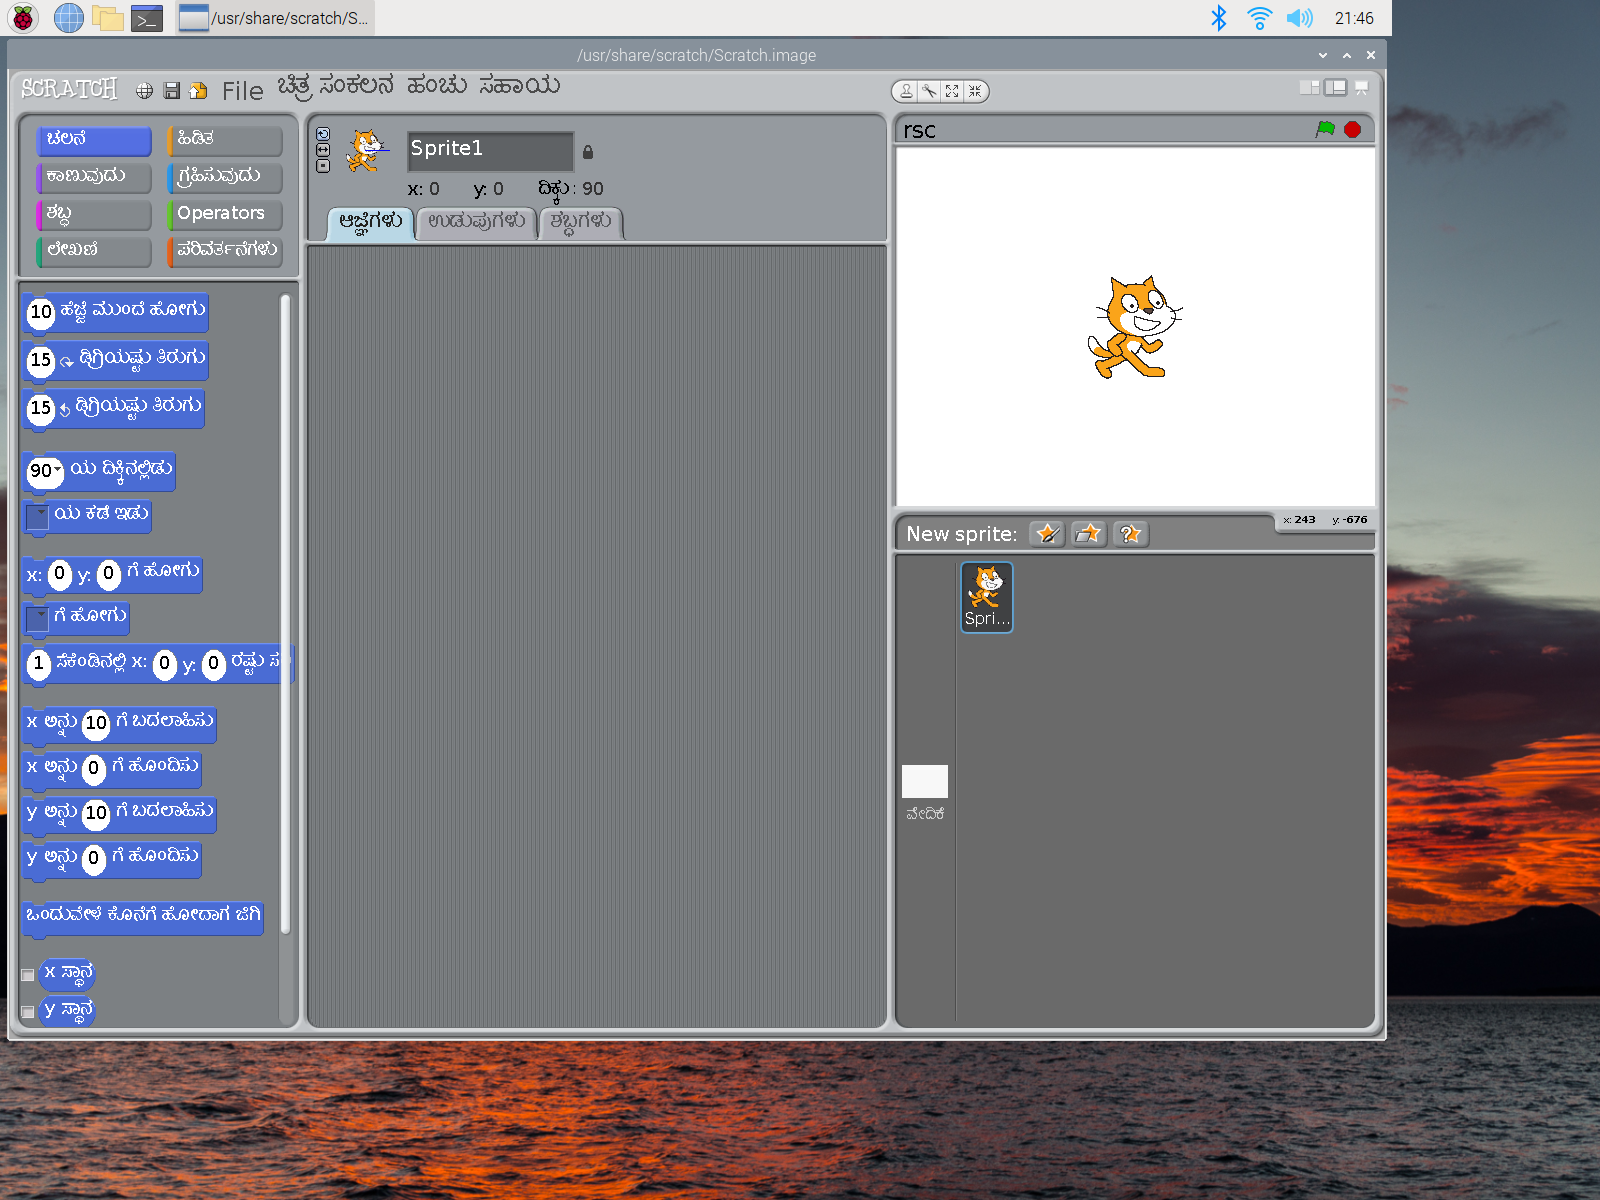
\includegraphics[scale=0.4]{ScratchScreen.pdf}};
\node at (4.4cm,2.2cm)(sprite_main){\Scratchy[0.11]};
\node at (-3.5cm,4.1cm)(sprite_top){\Scratchy[0.05]};
\node at (3cm,-0.5cm)(sprite_btm){\Scratchy[0.04]};
\node at (-6cm,5.5cm)(grp){ ಆಜ್ಞೆಗಳ ಗುಂಪುಗಳು};
\node at (-6cm,-5.6cm)(cmd){ ಚಲನೆ ಗುಂಪಿನ ಆಜ್ಞೆಗಳು};
\node at (-1cm,0)(scratch){ ಪ್ರೋಗ್ರಾಂ ತಯಾರಿಯ ಸ್ಥಳ};
\node at (4.4cm,1cm)(canvas){ ವೇದಿಕೆ};
\draw[->](cmd.north)--++(0.3cm,0.8cm);
\draw[->](grp.south)--++(0.3cm,-1cm);
\end{tikzpicture}
\caption{ಸ್ಕ್ರಾಚ್ ಸ್ಕ್ರೀನ್ ಹೀಗೆ ಕಾಣುತ್ತದೆ}
\label{ScratchScreen}
\end{figure}
\end{center}

ಸ್ಕ್ರಾಚ್ ಪ್ರಾರಂಭಿಸಿದಾಗ ಚಿತ್ರ \ref{ScratchScreen} ನಲ್ಲಿನಂತೆ ಕಾಣಿಸುತ್ತದೆ. ಕಂಪ್ಯೂಟರ್, ನಾವು ನೀಡುವ ಆಜ್ಞೆಗಳಂತೆ ಕೆಲಸ ಮಾಡುತ್ತದೆ.  ಸ್ಕ್ರಾಚ್ನಲ್ಲಿ ಕಂಪ್ಯೂಟರ್ಗೆ ನೀಡುವ ಆಜ್ಞೆಗಳನ್ನು ಮಾಡಿ ತೋರಿಸುವುದಕ್ಕೆ ಒಂದು ಬೆಕ್ಕು ಇದೆ. ಈ ಬೆಕ್ಕಿನ ಹೆಸರು ಸ್ಪ್ರಯ್ಟ್ ಎಂದು. ಸ್ಕ್ರಾಚ್ನಲ್ಲಿ ಸ್ಪ್ರಯ್ಟ್ಗೆ ನೀಡಬಹುದಾದ ಎಲ್ಲಾ ಆಜ್ಞೆಗಳನ್ನು ಎಂಟು ಗುಂಪುಗಳಲ್ಲಿ ವಿಂಗಡಿಸಲಾಗಿದೆ.  ಆಜ್ಞೆಗಳ ಗುಂಪು ಎಲ್ಲಿದೆ ಎಂದು ಚಿತ್ರದಲ್ಲಿ ಕಾಣಿರಿ. ಸಧ್ಯಕ್ಕೆ "ಚಲನೆ" ಮತ್ತು "ಹಿಡಿತ" ಎಂಬ ಎರಡು ಗುಂಪುಗಳಲ್ಲಿನ  ಆಜ್ಞೆಗಳನ್ನು ಬಳಸಿ ಪ್ರೋಗ್ರಾಂ ಬರೆಯುವುದನ್ನು ಕಲಿಯೋಣ.
\section{ಆರಂಭ}

ಮೊದಲಿಗೆ ನೀಲಿ ಬಣ್ಣದ "ಚಲನೆ" ಆಜ್ಞೆಗಳ ಗುಂಪನ್ನು ಒತ್ತಿ.  ನೀಲಿ ಬಣ್ಣದ ಚಲನೆ ಆಜ್ಞೆಗಳ ಕಂಡುಬರುತ್ತವೆ.  ಎಲ್ಲಾ ಚಲನೆ ಆಜ್ಞೆಗಳನ್ನು ಒಮ್ಮೆ ಪರಿಶೀಲಿಸಿ. ಈ ಆಜ್ಞೆಗಳನ್ನು  ಉಪಯೋಗೊಸಿಕೊಡು ಸ್ಪ್ರಯ್ಟ್ ಆನು ಹೇಗೆ ಕೆಲಸ ಮಾಡುವಂತೆ ಪ್ರೋಗ್ರಾಂ ಬರೆಯುವುದು ಎಂದು ಯೋಚಿಸಿ.  ಚಲನೆ ಗುಂಪಿನ ನಂತರ ಕೇಸರಿ ಬಣ್ಣದ "ಹಿಡಿತ" ಆಜ್ಞೆಗಳ ಗುಂಪನ್ನು ಒತ್ತಿ.  ಕೇಸರಿ ಬಣ್ಣದ ಹಿಡಿತ ಆಜ್ಞೆಗಳು ಕಂಡುಬರುತ್ತವೆ.  ಇದೇ ರೀತಿ ಬೇರೆ ಬೇರೆ ಗುಂಪನ್ನು ಒತ್ತಿ ಆ ಗುಂಪಿನ ಆಜ್ಞೆಗಳನ್ನು ಪರಿಶೀಲಿಸಿ.

ಪ್ರೋಗ್ರಾಂ ತಯಾರಿಸುವುದೆಂದರೆ ಈ ಹಲವು ಬಗೆಗಿನ ಆಜ್ಞೆಗಳನ್ನು ಒಂದಾದ ನಂತರ ಒಂದಂತೆ ಜೋಡಿಸಿ ನಮಗೆ ಬೇಕಾದ ಕೆಲಸ ಮಾಡಿಸಿಕೊಳ್ಳುವುದು. ಪ್ರೋಗ್ರಾಂ ತಯಾರಿಯ ಸ್ಥಳದಲ್ಲಿ ಆಜ್ಞೆಗಳನ್ನು ಜೋಡಿಸಿ ಪ್ರೋಗ್ರಾಂ ತಯಾರಿಸಬೇಕು. ಪ್ರೋಗ್ರಾಂನಲ್ಲಿ ನೀಡಿದ ಆಜ್ಞೆಯ ಪ್ರಕಾರ ಸ್ಪ್ರೈಟ್ ಕೆಲಸ ಮಾಡುತ್ತದೆ. ಉದಾಹರಣೆಗೆ “ಹತ್ತು ಹೆಜ್ಜೆ ಮುಂದೆ ಹೋಗು” ಎಂದು ಆಜ್ಞೆ ಮಾಡಿದರೆ ಅದು ಹತ್ತು ಹೆಜ್ಜೆ ಮುಂದೆ ಹೋಗುತ್ತದೆ. ನಂತರ “90 ಡಿಗ್ರಿ ಬಲಕ್ಕೆ ತಿರುಗು” ಎಂದರೆ ಬಲಕ್ಕೆ ತಿರುಗುತ್ತದೆ. ಇನ್ನೂ ಹಲವಾರು ವಿಧದ ಆಜ್ಞೆಗಳನ್ನೆಲ್ಲ ಮುಂದಕ್ಕೆ ಒಂದೊಂದಾಗಿ ತಿಳಿಯೋಣ.

\section{ಆಜ್ಞೆಗಳನ್ನು ಜೋಡಿಸುವುದು}
ಈಗ ಕೆಳಗಿನ ಸೂಚನೆಯಂತೆ ಮೌಸ್ ಉಪಯೊಗಿಸಿ ಮಾಡಿ ನೋಡಿ.  

\begin{enumerate}
\item{"ಚಲನೆ" ಗುಂಪನ್ನು ಒತ್ತಿ.}
\item{"ಚಲನೆ" ಗುಂಪಿನ ಆಜ್ಞೆಗಳನ್ನು ಒತ್ತಿ.}
\item{"ಚಲನೆ" ಗುಂಪಿನ ಆಜ್ಞೆಗಳಲ್ಲಿ ಒಂದನ್ನು ಪ್ರೋಗ್ರಾಂ ತಯಾರಿಯ ಸ್ಥಳದಲ್ಲಿ ತಂದಿರಿಸಿ.}
\item{ಪ್ರೋಗ್ರಾಂ ತಯಾರಿಯ ಸ್ಥಳದಲ್ಲಿರುವ ಆಜ್ಞೆಯನ್ನು ಅತ್ತಿತ್ತ ಜರುಗಿಸಿ.}
\item{ಪ್ರೋಗ್ರಾಂ ತಯಾರಿಯ ಸ್ಥಳದಲ್ಲಿರುವ ಆಜ್ಞೆಗೆ ಮತ್ತೊಂದು ಆಜ್ಞೆಯನ್ನು ಜೋಡಿಸಿ.}
\end{enumerate}

ಜೋಡಿಸುವಾಗ ಎರಡು ಆಜ್ಞೆಗಳು ಹತ್ತಿರ ಬರುತ್ತಿದಂತೆ ಒಂದು ಬಿಳಿ ಗೆರೆ ಕಣಿಸಿಕೊಳ್ಳುವುದನ್ನು ಗಮನಿಸಿ.  ಬಿಳಿ ಗೆರೆ ಕಂಡೊಡನೆ ಒತ್ತಿಟ್ಟುಕೊಂಡ ಮೌಸ್ ಬಿಟ್ಟರೆ ಆಜ್ಞೆಗಳು ಒಂದಕ್ಕೊಂದು ಜೋಡಿಸಿಕೊಳ್ಳುತ್ತವೆ.  ಜೋಡಿ ಆಜ್ಞೆಗಳನ್ನು ಅತ್ತಿತ್ತ ಜರುಗಿಸುವುದಕ್ಕೆ ಮೌಸ್  ಅನ್ನು ಎಲ್ಲಿ ಒತ್ತಿಟ್ಟುಕೊಂಡು ಜರುಗಿಸುತ್ತೇವೆ ಎಂಬುದಕ್ಕೆ ಗಮನ ಕೊಡಬೇಕು. ಜೋಡಿ ಆಜ್ಞೆಗಳಲ್ಲಿ ಮೇಲಿನ ಆಜ್ಞೆಯನ್ನು ಹಿಡಿದು ಅತ್ತಿತ್ತ ಜರುಗಿಸಿದರೆ ಒಟ್ಟು ಪ್ರೋಗ್ರಾಂ ಜರುಗುತ್ತದೆ.

\section{ಆಜ್ಞೆಗಳನ್ನು ಬಿಡಿಸುವುದು}
ಕಂಪ್ಯೂಟರ್ ಪ್ರೋಗ್ರಾಂ ತಯಾರಿಸುವಾಗ ತಪ್ಪುಗಳಾಗುವುದು ಬಹಳ ಸಹಜ. ಹಾಗೆ ತಪ್ಪಾದಾಗ ಅದನ್ನು ತಿದ್ದುವುದು ಹೇಗೆ? ಜೋಡಿ ಆಜ್ಞೆಗಳಲ್ಲಿ ಮೇಲಿನ ಆಜ್ಞೆಯನ್ನು ಹಿಡಿದು ಅತ್ತಿತ್ತ ಜರುಗಿಸಿದರೆ ಒಟ್ಟು ಪ್ರೋಗ್ರಾಂ ಜರುಗುತ್ತದೆ.ಆದರೆ ಕೆಳಗಿನ ಆಜ್ಞೆಯನ್ನು ಹಿಡಿದು ಜರುಗಿಸಿದರೆ ಅದು ಗುಂಪನ್ನು ಬಿಟ್ಟು ಬರುತ್ತದೆ. ಹೀಗೆ ತಪ್ಪಾದ ಆಜ್ಞೆಯನ್ನು ಹೊರತೆಗೆದು ಮತ್ತೆ ಆಜ್ಞೆಗಳ ಗುಂಪಿನಲ್ಲಿ ಬಿಟ್ಟರೆ ಅದು ಮಾಯವಾಗಿ ನಮಗೆ ಪ್ರೋಗ್ರಾಂ ತಿದ್ದಲು ಅವಕಾಶ ಸಿಗುತ್ತದೆ.  ಈಗ ಜೋಡಿಸಿದ  ಆಜ್ಞೆಗಳನ್ನು ಬಿಡಿಸಿ ನೋಡಿ.

\section{ಅಭ್ಯಾಸ}

\begin{figure}[h]
\begin{center}
\begin{Scratch}[1.2]
\scbox{\cb[w]{10}  ಹೆಜ್ಜೆ ಮುಂದೆ ಹೋಗು}{motion}
\scbox{\cb[w]{20}  ಹೆಜ್ಜೆ ಮುಂದೆ ಹೋಗು}{motion}
\scbox{\cb[w]{30}  ಹೆಜ್ಜೆ ಮುಂದೆ ಹೋಗು}{motion}
\scbox{\cb[w]{40}  ಹೆಜ್ಜೆ ಮುಂದೆ ಹೋಗು}{motion}
\scbox{\cb[w]{50}  ಹೆಜ್ಜೆ ಮುಂದೆ ಹೋಗು}{motion}
\scbox{\cb[w]{100}  ಹೆಜ್ಜೆ ಮುಂದೆ ಹೋಗು}{motion}
\end{Scratch}
\caption{ಮೌಸ್ ಬಳಸುವುದನ್ನು ಅಭ್ಯಾಸ ಮಾಡಲು ಹೀಗೆ ಜೋಡಿಸಿ,  ಬಿಡಿಸಿ}
\label{mouse1}
\end{center}
\end{figure}

\vspace{-0.5cm}
ಚಿತ್ರ \ref{mouse1} ನಲ್ಲಿನಂತೆ ಆಜ್ಞೆಗಳನ್ನು ಜೋಡಿಸಿ ಮತ್ತು ಬಿಡಿಸಿ ನೋಡಿ.  ಈ ಪ್ರೋಗ್ರಾಂನಂತೆ ಸ್ಪ್ರೈಟ್ ಕೆಲಸ ಮಾಡಿದರೆ ಒಟ್ಟು ಎಷ್ಟು ಹೆಜ್ಜೆ ಮುಂದೆ ಹೋಗಬಹುದು ಎಂದು ಒಮ್ಮೆ ಯೊಚಿಸಿ.

\begin{figure}[h]
\begin{center}
\begin{Scratch}[1.2]
\boucle{\cb[w]{1} ಮರುಕಳಿಸು}{1}{1}
\scbox{\cb[w]{10}  ಹೆಜ್ಜೆ ಮುಂದೆ ಹೋಗು}{motion}
\end{Scratch}
\caption{ಮರುಕಳಿಸು ಆಜ್ಞೆಯ ಒಳಗೆ ಚಲನೆ ಗುಂಪಿನ ಆಜ್ಞೆಗಳನ್ನು ಜೋಡಿಸಿ, ಬಿಡಿಸಿ}
\label{mouse2}
\end{center}
\end{figure}

ಚಿತ್ರ \ref{mouse2} ನಲ್ಲಿನಂತೆ  ಹಿಡಿತ ಗುಂಪಿನಿಂದ ಮರುಕಳಿಸು ಎಂಬ ಆಜ್ಞೆಯನ್ನು ತಂದು ಅದರೊಳಗೆ ಚಲನೆ ಗುಂಪಿನ ಆಜ್ಞೆಯನ್ನು ಜೋಡಿಸಿ.  ಇದೇ ರೀತಿ ಇನ್ನೂ ಹಲವು ಚಲನೆ ಗುಂಪಿನ ಆಜ್ಞೆಗಳನ್ನು ತಂದು  ಜೋಡಿಸಿ ನೋಡಿ. ಈ ಬಾರಿಯೂ,  ಜೋಡಿಸುವಾಗ ಎರಡು ಆಜ್ಞೆಗಳು ಹತ್ತಿರ ಬರುತ್ತಿದಂತೆ ಒಂದು ಬಿಳಿ ಗೆರೆ ಕಣಿಸಿಕೊಳ್ಳುವುದನ್ನು ಗಮನಿಸಿ.  ಬಿಳಿ ಗೆರೆ ಕಂಡೊಡನೆ ಒತ್ತಿಟ್ಟುಕೊಂಡ ಮೌಸ್ ಬಿಟ್ಟರೆ ಆಜ್ಞೆಗಳು ಜೋಡಿಸಿಕೊಳ್ಳುತ್ತವೆ.  ಈಗ ಮರುಕಳಿಸು ಆಜ್ಞೆಯ ಒಳಗಿನಿಂದ ಚಲನೆ ಗುಂಪಿನ ಆಜ್ಞೆಗಳನ್ನು ಬಿಡಿಸಿ ನೋಡಿ.  ಬಿಡಿಸದೆ ಒಟ್ಟು ಪ್ರೋಗ್ರಾಂ ಅನ್ನು ಅತ್ತಿತ್ತ ಜರುಗಿಸುವುದು ಹೇಗೆ ಎಂದು ಕಲಿಯಿರಿ. 

ಈಗ ಚಿತ್ರ \ref{mouse1} ನಲ್ಲಿನ ಎಲ್ಲಾ ಆಜ್ಞೆಗಳನ್ನು ಮರುಕಳಿಸು ಆಜ್ಞೆಯ ಒಳಗೆ ಜೋಡಿಸಿ ಮತ್ತು ಒಂದೊಂದಾಗಿ ಬಿಡಿಸುವುದನ್ನು ಪ್ರಯತ್ನಿಸಿ.

ಚಲನೆ ಗುಂಪಿನ ಆಜ್ಞೆಗಳಲ್ಲಿ ಸಂಖ್ಯೆಗಳಿವೆ. ಇವನ್ನು ಬದಲಾಯಿಸಬೇಕಾದರೆ ಆ ಸಂಖ್ಯೆಯ ಮೇಲೆ ಮೌಸ್ನಿಂದ  ಒತ್ತಿ.  ಆಗ ಸಂಖ್ಯೆಯ ಬಿಳಿ ಹಿಂಭಾಗ, ನೀಲಿ ಬಣ್ಣಕ್ಕೆ ತಿರುಗುತ್ತದೆ. ಹೀಗಿದ್ದಾಗ ಕೀಲಿಮಣೆಯಲಿನ  (\textenglish{keyboard}) ಸಂಖ್ಯೆಗಳ್ಳನ್ನು ಒತ್ತಿದರೆ ಆ ಸಂಖ್ಯೆಗಳು, ಆಜ್ಞೆಗೆ ಸೇರಿಕೊಳ್ಳುತ್ತದೆ. ಇದನ್ನೂ ಅಭ್ಯಾಸ ಮಾಡಿ. 


\chapter{ಮೊದಲ ಪ್ರೋಗ್ರಾಂ}
ಕಂಪ್ಯೂಟರ್, ನಾವು ನೀಡುವ ಆಜ್ಞೆಗಳಂತೆ ಯಥಾವತ್ತಾಗಿ ಕೆಲಸ ಮಾಡುತ್ತದೆ.  ನಾವು ಹಿಂದಿನ ಅಧ್ಯಾಯದಲ್ಲಿ ಸ್ಕ್ರಾಚ್ ಸ್ಕ್ರೀನ್ ಅನ್ನು ನೋಡಿದೆವು. ಈಗ ನಾವು ಕೊಡುವ ಆಜ್ಞೆಗಳಿಂದಾಗಿ ಸ್ಪ್ರಯ್ಟ್  ಏನೆಲ್ಲಾ ಕೆಲಸ ಮಾಡುವುದೆಂದು ನೋಡೋಣ.  ಮೊದಲಿಗೆ "ಚಲನೆ" ಮತ್ತು "ಹಿಡಿತ" ಗುಂಪುಗಳಲ್ಲಿನ  ಆಜ್ಞೆಗಳನ್ನು ಬಳಸಿ ಸ್ಪ್ರಯ್ಟ್ ನಿಂದ ಕೆಲಸ ಮಾಡಿಸೋಣ. 



\section{ಮುಂದೆ ಹೋಗು}
\begin{figure}[h]
\begin{center}
\begin{multicols}{2}
\begin{Scratch}[1]
\beginbox{}
\scbox{\cb[w]{10} ಹೆಜ್ಜೆ ಮುಂದೆ ಹೋಗು}{motion}
\end{Scratch}

\begin{tikzpicture}
\node[doc] (x) (inst1){
ಒತ್ತಿದಾಗ\\
10  ಹೆಜ್ಜೆ ಮುಂದೆ ಹೋಗು
};
\end{tikzpicture}
\end{multicols}
\begin{tikzpicture}
\node at (0,0)[rotate=0, opacity=0.2](s1){\Scratchy[0.2]};
\draw[->](s1.east)--++(0.5cm,0)node(newcoord){};
\node at ([shift={(1cm,0)}]newcoord)[rotate=0, opacity=1](s2){\Scratchy[0.2]};
\end{tikzpicture}
\end{center}

\caption{ಮೊದಲನೆ ಪ್ರೋಗ್ರಾಂ: ಸ್ಪ್ರಯ್ಟ್  ಅನ್ನು ಮುಂದೆ ಹೋಗಿಸುವುದು}
\label{program1}
\end{figure}

\vspace{-0.5cm}
ಮೊದಲನೆಯದಾಗಿ ಹಿಡಿತ ಗುಂಪಿನ "ಒತ್ತಿದಾಗ" ಎಂಬ ಆಜ್ಞೆಯನ್ನು ಪ್ರೋಗ್ರಾಂ ತಯಾರಿಯ ಜಾಗದಲ್ಲಿರಿಸೋಣ.  ಈ ಆಜ್ಞೆ ಏನು ಮಾಡುವುದೆಂದರೆ,  ನೀವು ಮೌಸ್ನಿಂದ ವೇದಿಕೆಯ ಮೇಲಿನ ಹಸಿರು ಧ್ವಜವನ್ನು ಒತ್ತಿದಾಗ, ಈ ಆಜ್ಞೆಯ ಕೆಳಗಿನ ಪ್ರೋಗ್ರಾಮಿನಂತೆ ಸ್ಪ್ರಯ್ಟ್ ನಿಂದ ಕೆಲಸ ಮಾಡಿಸುತ್ತದೆ. ಈಗ, "ಒತ್ತಿದಾಗ" ಆಜ್ಞೆಯ ಕೆಳಗೆ “ಹತ್ತು ಹೆಜ್ಜೆ ಮುಂದೆ ಹೋಗು” ಎಂದು ಆಜ್ಞೆಯನ್ನು ಚಲನೆ ಗುಂಪಿನಿಂದ ತಂದು ಜೋಡಿಸಿ.  ನಿಮ್ಮ ಮೊದಲನೆ ಪ್ರೋಗ್ರಾಂ ಈಗ ಚಿತ್ರ \ref{program1}  ಎಡಭಾಗದಂತೆ ಕಾಣಬೇಕು.  ಈಗ ವೇದಿಕೆಯ ಮೇಲಿನ ಹಸಿರು ಧ್ವಜವನ್ನು ಒತ್ತಿ,  ಸ್ಪ್ರಯ್ಟ್ ಹತ್ತು ಹೆಜ್ಜೆ ಮುಂದೆ ಹೋಗುವುದೇ ಪರಿಶೀಲಿಸಿ.  ಚಿತ್ರ \ref{program1}ರ ಕೆಳಭಾಗದಲ್ಲಿ ತೋರಿಸಿರುವಂತೆ ಸ್ಪ್ರಯ್ಟ್ ತಾನಿದ್ದಲ್ಲಿಂದ ಹತ್ತು ಹೆಜ್ಜೆ ಮುಂದೆ ಹೋಗಿರಬೇಕು. 

ಪ್ರೋಗ್ರಾಂಗಳನ್ನು ಸ್ಕ್ರಾಚ್ನಲ್ಲಿ ಪ್ರಯತ್ನಿಸುವ ಮುನ್ನ ಅದರಿಂದ ಏನು ಕೆಲಸ ಆಗಬೇಕು ಎನ್ನುವುದನ್ನು ಮನವರಿಕೆ ಮಾಡಿಕೊಂಡಿರಬೇಕು. ಹೀಗೆ ಮನವರಿಕೆ ಮಾಡಿಕೊಳ್ಳುವುದಕ್ಕೆ ನಾವು ಮೊದಲು ಪುಸ್ತಕದಲ್ಲಿ ಪ್ರೋಗ್ರಾಂಗಳನ್ನು ಬರೆದು ಅವು ಹೇಗೆ ಕೆಲಸ ಮಾಡಬಹುದೆಂದು ಯೋಚಿಸಬಹುದು.  ಈ ಮೊದಲನೆ ಪ್ರೋಗ್ರಾಂಗೆ ಚಿತ್ರ \ref{program1} ಬಲಭಾಗದಲ್ಲಿರುವಂತೆ ಪುಸ್ತಕದಲ್ಲಿ  ಬರೆದುಕೊಳ್ಳಬಹುದು.  ಹೀಗೆ ಅಭ್ಯಾಸ ಮಾಡುವುದರಿಂದ, ನಮಗೆ ಕಂಪ್ಯೂಟರ್ ಸಿಕ್ಕ ಬಳಿಕ ಅದನ್ನು ಉಪಯುಕ್ತ ರೀತಿಯಲ್ಲಿ ಬಳಸಬಹುದು. 

\section{ಮುಂದೆ ಹೋಗಿ ತಿರುಗು}
\label{wait}
\begin{figure}[h]
\begin{center}
\begin{multicols}{2}
\begin{Scratch}[1]
\beginbox{}
\scbox{\cb[w]{100} ಹೆಜ್ಜೆ ಮುಂದೆ ಹೋಗು}{motion}
\turnbox{1}{90}{ಡಿಗ್ರಿಯಷ್ಟು ತಿರುಗು}
\end{Scratch}

\begin{tikzpicture}
\node[doc] (x) (inst1){
ಒತ್ತಿದಾಗ\\
100  ಹೆಜ್ಜೆ ಮುಂದೆ ಹೋಗು\\
90$‌^\circ$ ಬಲಕ್ಕೆ  ತಿರುಗು
};
\end{tikzpicture}

\end{multicols}

\begin{tikzpicture}
\node at (0,0)[rotate=0, opacity=0.2](s1){\Scratchy[0.2]};
\draw[->](s1.east)--++(2cm,0)node(newcoord){};
\node at ([shift={(1cm,0)}]newcoord)[rotate=-90, opacity=1](s2){\Scratchy[0.2]};
\end{tikzpicture}
\end{center}
\caption{ಸ್ಪ್ರಯ್ಟ್ ಮುಂದೆ ಹೋದ ಮೇಲೆ ಬೇಕಾದಂತೆ ತಿರುಗಿಸುವುದು}
\label{program2}
\end{figure}

ಸ್ಪ್ರಯ್ಟ್ ಮುಂದೆ ಹೋದ ಮೇಲೆ ನಮಗೆ ಬೇಕಾದಂತೆ ತಿರುಗಿಸುವುದು ಹೇಗೆ ಎಂದು ನೋಡೋಣ. ಮೊದಲಿನಂತೆ, ಹಿಡಿತ ಗುಂಪಿನ "ಒತ್ತಿದಾಗ" ಎಂಬ ಆಜ್ಞೆಯನ್ನು ಪ್ರೋಗ್ರಾಂ ತಯಾರಿಯ ಜಾಗದಲ್ಲಿರಿಸಿ, ಅದಕ್ಕೆ “ಹತ್ತು ಹೆಜ್ಜೆ ಮುಂದೆ ಹೋಗು” ಎಂಬ ಆಜ್ಞೆಯನ್ನು ಚಲನೆ ಗುಂಪಿನಿಂದ ತಂದು ಜೋಡಿಸಿ.  ಈ ಆಜ್ಞೆಯಲ್ಲಿ 10 ಸಂಖ್ಯೆಯನ್ನು 100 ಕ್ಕೆ ಬದಲಾಯಿಸಿ.  ಇವೆರಡರ ಕೆಳಗೆ,  "90 ಡಿಗ್ರಿಯಷ್ಟು ತಿರುಗು" ಎಂಬ ಆಜ್ಞೆಯನ್ನು ತಂದು ಜೋಡಿಸಿ.  ಈ ಆಜ್ಞೆಯಲ್ಲಿ ತಿರುಗುವ ದಿಕ್ಕು ಯವುದಿದೆ ಎಂದು ಪರೀಕ್ಷಿಸಿಕೊಳ್ಳಿ. ನಿಮ್ಮ ಪ್ರೋಗ್ರಾಂ ಈಗ ಚಿತ್ರ \ref{program2}  ಎಡಭಾಗದಂತೆ ಕಾಣಬೇಕು.    ವೇದಿಕೆಯ ಮೇಲಿನ ಹಸಿರು ಧ್ವಜವನ್ನು ಒತ್ತಿ,  ಸ್ಪ್ರಯ್ಟ್ ನೂರು ಹೆಜ್ಜೆ ಮುಂದೆ ಹೋಗಿ, ಬಲಕ್ಕೆ ತಿರುಗುವುದೇ, ಪರಿಶೀಲಿಸಿ.  ಚಿತ್ರ \ref{program2}ರ ಕೆಳಭಾಗದಲ್ಲಿ ತೋರಿಸಿರುವಂತೆ ಸ್ಪ್ರಯ್ಟ್ ತಾನಿದ್ದಲ್ಲಿಂದ ನೂರು ಹೆಜ್ಜೆ ಮುಂದೆ ಹೋಗಿ ಬಲಕ್ಕೆ 90 ಡಿಗ್ರಿ ತಿರುಗಿರಬೇಕು.  ಚಿತ್ರ \ref{program2}ನ ಬಲಭಾಗದಲ್ಲಿರುವಂತೆ  ಅಭ್ಯಾಸಕ್ಕಾಗಿ ಪುಸ್ತಕದಲ್ಲಿ  ಪ್ರೋಗ್ರಾಂ ಅನ್ನು ಸರಳವಾಗಿ ಬರೆದುಕೊಳ್ಳಬಹುದು. 

ಈಗ ಕಲಿತಿರುವ ಆಜ್ಞೆಗಳನ್ನೇ ಉಪಯೋಗಿಸಿಕೊಂಡು ಒಂದು ಕುತೂಹಲಕಾರಿ ಪ್ರೋಗ್ರಾಂ ಅನ್ನು ರಚಿಸೋಣ.  ಈಗ ಚಿತ್ರ \ref{program3}  ಎಡಭಾಗದಂತೆ ಆಜ್ಞೆಗಳನ್ನು ತಂದು ಜೋಡಿಸಿ.    

\begin{figure}[h]
\begin{center}
\begin{multicols}{2}
\begin{Scratch}[1]
\beginbox{}
\scbox{\cb[w]{100} ಹೆಜ್ಜೆ ಮುಂದೆ ಹೋಗು}{motion}
\turnbox{1}{90}{ಡಿಗ್ರಿಯಷ್ಟು ತಿರುಗು}
\scbox{\cb[w]{100} ಹೆಜ್ಜೆ ಮುಂದೆ ಹೋಗು}{motion}
\turnbox{1}{90}{ಡಿಗ್ರಿಯಷ್ಟು ತಿರುಗು}
\scbox{\cb[w]{100} ಹೆಜ್ಜೆ ಮುಂದೆ ಹೋಗು}{motion}
\turnbox{1}{90}{ಡಿಗ್ರಿಯಷ್ಟು ತಿರುಗು}
\scbox{\cb[w]{100} ಹೆಜ್ಜೆ ಮುಂದೆ ಹೋಗು}{motion}
\end{Scratch}

\begin{tikzpicture}
\node[doc] (x) (inst1){
ಒತ್ತಿದಾಗ\\
100  ಹೆಜ್ಜೆ ಮುಂದೆ ಹೋಗು\\
90$‌^\circ$ ಬಲಕ್ಕೆ  ತಿರುಗು\\
100  ಹೆಜ್ಜೆ ಮುಂದೆ ಹೋಗು\\
90$‌^\circ$ ಬಲಕ್ಕೆ  ತಿರುಗು\\
100  ಹೆಜ್ಜೆ ಮುಂದೆ ಹೋಗು\\
90$‌^\circ$ ಬಲಕ್ಕೆ  ತಿರುಗು\\
100  ಹೆಜ್ಜೆ ಮುಂದೆ ಹೋಗು
};
\end{tikzpicture}

\end{multicols}

\begin{tikzpicture}
\node at (0,0)[rotate=0, opacity=0.2](s1){\Scratchy[0.2]};
\draw[->](s1.east)--++(2cm,0)node(newcoord){};
\node at ([shift={(1cm,0)}]newcoord)[rotate=-90, opacity=0.2](s2){\Scratchy[0.2]};
\draw[->](s2.east)--++(0,-2cm)node(newcoord){};
\node at ([shift={(0,-1cm)}]newcoord)[rotate=-180, opacity=0.2](s3){\Scratchy[0.2]};
\draw[->](s3.east)--++(-2cm,0cm)node(newcoord){};
\node at ([shift={(-1cm,0)}]newcoord)[rotate=90, opacity=0.2](s4){\Scratchy[0.2]};
\draw[->](s4.east)--++(0,2cm)node(newcoord){};
\node at ([shift={(0,1cm)}]newcoord)[rotate=90, opacity=1](s2){\Scratchy[0.2]};
\end{tikzpicture}
\end{center}
\caption{ಸ್ಪ್ರಯ್ಟ್ ಅನ್ನು ಚೌಕಾಕಾರವಾಗಿ ಚಲಾಯಿಸುವುದು}
\label{program3}
\end{figure}

ನಿಮ್ಮ ಪ್ರೋಗ್ರಾಂ ಈಗ ಚಿತ್ರ \ref{program3}  ಎಡಭಾಗದಂತೆ ಕಾಣಬೇಕು.   ಪ್ರೋಗ್ರಾಂ ಅನ್ನು  ಚಲಾಯಿಸಿ (ವೇದಿಕೆಯ ಮೇಲಿನ ಹಸಿರು ಧ್ವಜವನ್ನು ಒತ್ತಿ),  ಸ್ಪ್ರಯ್ಟ್ ಮುಂದೆ ಹೋಗಿ, ಬಲಕ್ಕೆ ತಿರುಗುವುದನ್ನು ನಾಲ್ಕು ಬಾರಿ ಮಾಡುವುದೇ ಎಂದು ಪರಿಶೀಲಿಸಿ.  ಚಿತ್ರ \ref{program3}ರ ಕೆಳಭಾಗದಲ್ಲಿ ತೋರಿಸಿರುವಂತೆ ಸ್ಪ್ರಯ್ಟ್ ತಾನಿದ್ದಲ್ಲಿಂದ ನೂರು ಹೆಜ್ಜೆ ಮುಂದೆ ಹೋಗಿ ಬಲಕ್ಕೆ 90 ಡಿಗ್ರಿ ನಾಲ್ಕು ಬಾರಿ ತಿರುಗಿರಬೇಕು.  ಸ್ಪ್ರಯ್ಟ್ ಹೀಗೆ ಹಂತ ಹಂತವಾಗಿ ಕೆಲಸ ಮಾಡುವುದು ನಮ್ಮ ಕಣ್ಣಿಗೆ ಕಾಣುತ್ತದೆಯೇ? ಏಕೆ ಕಾಣುವುದಿಲ್ಲ ಎಂದು ಒಮ್ಮೆ ಯೋಚಿಸಿ. 

ಚಿತ್ರ \ref{program3}ನ ಬಲಭಾಗದಲ್ಲಿರುವಂತೆ  ಈ ಪ್ರೋಗ್ರಾಂ ಆನ್ನು ಪುಸ್ತಕದಲ್ಲಿ  ಸರಳವಾಗಿ ಬರೆದುಕೊಳ್ಳಬಹುದು.   ಇದರಲ್ಲಿ ಗಮನಿಸಿ, ಸ್ಪ್ರಯ್ಟ್  ತಾನು ಮೊದಲಿದ್ದ ದಿಕ್ಕಿನಲ್ಲಿ ಮುಖ ಮಾಡಿ ನಿಂತಿಲ್ಲ. ಏಕೆ? ಅದು ಮೊದಲಿದ್ದ ದಿಕ್ಕಿನಲ್ಲಿ ಮುಖ ಮಾಡಿ ನಿಲ್ಲಬೇಕಾದರೆ ಪ್ರೋಗ್ರಾಂ ಅನ್ನು ಹೇಗೆ ಬದಲಾಯಿಸ ಬೇಕು? ಈ ಸವಾಲು  ಒದುಗರ ಪ್ರಯತ್ನಕ್ಕೆ.

\section{ಕಾಯುವುದು}
ಕಂಪ್ಯೂಟರ್, ನಾವು ನೀಡುವ ಆಜ್ಞೆಗಳಂತೆ ಯಥಾವತ್ತಾಗಿ ಅತಿವೇಗವಾಗಿ ಕೆಲಸ ಮಾಡಿಬಿಡುತ್ತದೆ. ಹಾಗಾಗಿ ಅದು ಹಂತ ಹಂತವಾಗಿ ಕೆಲಸ ಮಾಡುವುದು ನಮ್ಮ ಕಣ್ಣಿಗೆ ಕಾಣುವುದಿಲ್ಲ.  ನಮಗೆ ಕಾಣಿಸಬೇಕಾದರೆ,  ಪ್ರೋಗ್ರಾಂ ಆನ್ನು ನಮಗೆ ಬೇಕಾದ ಹಂತಗಳಲ್ಲಿ ತಡೆದು ಕಾಯಿಸಬೇಕು - ಹೇಗೆ ಎಂದು ಈಗ ನೋಡೋಣ.


\begin{figure}[h]
\begin{center}
\begin{multicols}{2}
\begin{Scratch}[1]
\beginbox{}
\scbox{\cb[w]{100} ಹೆಜ್ಜೆ ಮುಂದೆ ಹೋಗು}{motion}
\scbox{\cb[w]{1}  ಸೆಕೆಂಡುಗಳಷ್ಟು   ಕಾಯಬೇಕು}{control}
\turnbox{1}{90}{ಡಿಗ್ರಿಯಷ್ಟು ತಿರುಗು}
\scbox{\cb[w]{1}  ಸೆಕೆಂಡುಗಳಷ್ಟು   ಕಾಯಬೇಕು}{control}
\scbox{\cb[w]{100} ಹೆಜ್ಜೆ ಮುಂದೆ ಹೋಗು}{motion}
\scbox{\cb[w]{1}  ಸೆಕೆಂಡುಗಳಷ್ಟು   ಕಾಯಬೇಕು}{control}
\turnbox{1}{90}{ಡಿಗ್ರಿಯಷ್ಟು ತಿರುಗು}
\scbox{\cb[w]{1}  ಸೆಕೆಂಡುಗಳಷ್ಟು   ಕಾಯಬೇಕು}{control}
\scbox{\cb[w]{100} ಹೆಜ್ಜೆ ಮುಂದೆ ಹೋಗು}{motion}
\scbox{\cb[w]{1}  ಸೆಕೆಂಡುಗಳಷ್ಟು   ಕಾಯಬೇಕು}{control}
\turnbox{1}{90}{ಡಿಗ್ರಿಯಷ್ಟು ತಿರುಗು}
\scbox{\cb[w]{1}  ಸೆಕೆಂಡುಗಳಷ್ಟು   ಕಾಯಬೇಕು}{control}
\scbox{\cb[w]{100} ಹೆಜ್ಜೆ ಮುಂದೆ ಹೋಗು}{motion}
\scbox{\cb[w]{1}  ಸೆಕೆಂಡುಗಳಷ್ಟು   ಕಾಯಬೇಕು}{control}
\turnbox{1}{90}{ಡಿಗ್ರಿಯಷ್ಟು ತಿರುಗು}
\end{Scratch}

\begin{tikzpicture}
\node[doc] (x) (inst1){
ಒತ್ತಿದಾಗ\\
100  ಹೆಜ್ಜೆ ಮುಂದೆ ಹೋಗು\\
1 ಸೆಕೆಂಡುಗಳಷ್ಟು   ಕಾಯಬೇಕು\\
90$‌^\circ$ ಬಲಕ್ಕೆ  ತಿರುಗು\\
1 ಸೆಕೆಂಡುಗಳಷ್ಟು   ಕಾಯಬೇಕು\\
100  ಹೆಜ್ಜೆ ಮುಂದೆ ಹೋಗು\\
1 ಸೆಕೆಂಡುಗಳಷ್ಟು   ಕಾಯಬೇಕು\\
90$‌^\circ$ ಬಲಕ್ಕೆ  ತಿರುಗು\\
1 ಸೆಕೆಂಡುಗಳಷ್ಟು   ಕಾಯಬೇಕು\\
100  ಹೆಜ್ಜೆ ಮುಂದೆ ಹೋಗು\\
1 ಸೆಕೆಂಡುಗಳಷ್ಟು   ಕಾಯಬೇಕು\\
90$‌^\circ$ ಬಲಕ್ಕೆ  ತಿರುಗು\\
1 ಸೆಕೆಂಡುಗಳಷ್ಟು   ಕಾಯಬೇಕು\\
100  ಹೆಜ್ಜೆ ಮುಂದೆ ಹೋಗು\\
1 ಸೆಕೆಂಡುಗಳಷ್ಟು   ಕಾಯಬೇಕು\\
90$‌^\circ$ ಬಲಕ್ಕೆ  ತಿರುಗು
};
\end{tikzpicture}
\end{multicols}
\end{center}
\caption{ಸ್ಪ್ರಯ್ಟ್ ಆನು ಹಂತ ಹಂತವಾಗಿ ಕಾಯ್ದಿರಿಸಿ ಪ್ರೋಗ್ರಾಮ್ಮನ್ನು ವಿಶ್ಲೇಷಿಸುವುದು}
\label{program4}
\end{figure}

ಇದಕ್ಕೆ "ಹಿಡಿತ" ಗುಂಪಿನ "1 ಸೆಕೆಂಡುಗಳಷ್ಟು   ಕಾಯಬೇಕು" ಎನ್ನುವ ಆಜ್ಞೆಯನ್ನು ಬಳಸಬೇಕು.  ಈ ಆಜ್ಞೆಯನ್ನು ಬಳಸಿ ಚಿತ್ರ \ref{program4}ರ ಎಡಭಾಗದಲ್ಲಿ ತೋರಿಸಿರುವಂತೆ ಪ್ರೋಗ್ರಾಂ ಅನ್ನು ತಯಾರಿಸಿ.  ಸಂಕ್ಷಿಪ್ತವಾಗಿ ಹೇಳುವುದಾದರೆ, ಚಿತ್ರ \ref{program3}ರ ಪ್ರೋಗ್ರಾಮಿಗೆ ಒಂದೊಂದು ಹಂತದ ಮಧ್ಯೆಯೂ 1 ಸೆಕೆಂಡುಗಳಷ್ಟು   ಕಾಯುವ ಆಜ್ಞೆಯನ್ನು ಬಳಸಬೇಕು.  ಪ್ರೋಗ್ರಾಂ ಅನ್ನು  ಚಲಾಯಿಸಿ (ವೇದಿಕೆಯ ಮೇಲಿನ ಹಸಿರು ಧ್ವಜವನ್ನು ಒತ್ತಿ),  ಸ್ಪ್ರಯ್ಟ್ ಮುಂದೆ ಹೋಗಿ, 1 ಸೆಕೆಂಡುಗಳಷ್ಟು ಕಾದು ಬಲಕ್ಕೆ ತಿರುವುದನ್ನು ನಾಲ್ಕು ಬಾರಿ ಮಾಡುವುದೇ ಎಂದು ಪರಿಶೀಲಿಸಿ.  ಇದೇ ರೀತಿ ಕಂಪ್ಯೂಟರ್, ನಮ್ಮ ಆಜ್ಞೆಗಳನ್ನು ಅತಿವೇಗವಾಗಿ ನಿರ್ವಹಿಸುವಾಗ, ಪ್ರೋಗ್ರಾ ಮ್ಮನ್ನು ವಿಶ್ಲೇಷಿಸಬೇಕಾದರೆ,  ನಮಗೆ ಬೇಕಾದ ಹಂತಗಳಲ್ಲಿ ತಡೆದು ಕಾಯಿಸಬೇಕು.

ಚಿತ್ರ \ref{program3}ನ ಬಲಭಾಗದಲ್ಲಿರುವಂತೆ  ಈ ಪ್ರೋಗ್ರಾಂ ಆನ್ನು ಪುಸ್ತಕದಲ್ಲಿ  ಸರಳವಾಗಿ ಬರೆದುಕೊಳ್ಳಬಹುದು.   ಈಗ ಗಮನಿಸಿ, ಸ್ಪ್ರಯ್ಟ್  ತಾನು ಮೊದಲಿದ್ದ ದಿಕ್ಕಿನಲ್ಲಿಯೇ ಮುಖ ಮಾಡಿ ನಿಂತಿದೆ. 

\section{ಅಭ್ಯಾಸ }
\begin{enumerate}
\item{ಸ್ಪ್ರಯ್ಟ್ 200 ಹೆಜ್ಜೆ ಮುಂದೆ ಹೋಗುವಾಗ ಮಧ್ಯದಲ್ಲಿ ಒಮ್ಮೆ ಹಿಂದಕ್ಕೆ ತಿರುಗಿ ನೋಡಿ ಹೋಗುವಂತೆ ಪ್ರೋಗ್ರಾಂ ಬರೆಯಿರಿ. ಮೊದಲು ಪುಸ್ತಕದಲ್ಲಿ ಪ್ರಯತ್ನಿಸಿ ನಂತರ ಸ್ಕ್ರಾಚ್ನಲ್ಲಿ ಮಾಡಿ ನೋಡಿ. }


\begin{figure}[h]
\begin{center}
\begin{tikzpicture}
\node at (0,0)[rotate=0, opacity=0.2](s1){\Scratchy[0.2]};
\draw[->](s1.east)--++(2cm,0)node(newcoord){};
\node at ([shift={(1cm,0)}]newcoord)[rotate=-180, opacity=0.4](s2){\Scratchy[0.2]};
\node at ([shift={(1cm,0)}]newcoord)[rotate=0, opacity=0.6](s3){\Scratchy[0.2]};
\draw[->](s3.east)--++(2cm,0cm)node(newcoord){};
\node at ([shift={(1cm,0)}]newcoord)[rotate=0, opacity=1](s4){\Scratchy[0.2]};
\draw [->](s2.south)arc(80:-90:1.3cm);
\end{tikzpicture}
\end{center}
\caption{ಸ್ಪ್ರಯ್ಟ್ ಹಿಂದಿರುಗಿ ನೋಡಿ ಮುಂದೆ ಹೋಗುವುದು}
\label{program5}
\end{figure}

\item{ಸ್ಪ್ರಯ್ಟ್ 200 ಹೆಜ್ಜೆ ಮುಂದೆ ಹೋಗುವಾಗ ಮಧ್ಯದಲ್ಲಿ ಒಮ್ಮೆ ಕೆಳಕ್ಕೆ ನೋಡಿ ಹೋಗುವಂತೆ ಪ್ರೋಗ್ರಾಂ ಬರೆಯಿರಿ.  ಮೊದಲು ಪುಸ್ತಕದಲ್ಲಿ ಪ್ರಯತ್ನಿಸಿ ನಂತರ ಸ್ಕ್ರಾಚ್ನಲ್ಲಿ ಮಾಡಿ ನೋಡಿ. }


\begin{figure}[h]
\begin{center}

\begin{tikzpicture}
\node at (0,0)[rotate=0, opacity=0.2](s1){\Scratchy[0.2]};
\draw[->](s1.east)--++(2cm,0)node(newcoord){};
\node at ([shift={(1cm,0)}]newcoord)[rotate=-90, opacity=0.4](s2){\Scratchy[0.2]};
\node at ([shift={(1cm,0)}]newcoord)[rotate=0, opacity=0.6](s3){\Scratchy[0.2]};
\draw[->](s3.east)--++(2cm,0cm)node(newcoord){};
\node at ([shift={(1cm,0)}]newcoord)[rotate=0, opacity=1](s4){\Scratchy[0.2]};
\draw [->](s2.west)arc(80:0:1.5cm);
\end{tikzpicture}
\end{center}
\caption{ಸ್ಪ್ರಯ್ಟ್ ಕೆಳಗೆ ನೋಡಿ ಮುಂದೆ ಹೋಗುವುದು}
\label{program6}
\end{figure}

\item{ಸ್ಪ್ರಯ್ಟ್ 300 ಹೆಜ್ಜೆ ಮುಂದೆ ಹೋಗುವಾಗ ಮಧ್ಯದಲ್ಲಿ ಒಮ್ಮೆ ಪಲ್ಟಿ  ಹೊಡೆಯುವಂತೆ ಪ್ರೋಗ್ರಾಂ ಬರೆಯಿರಿ. }


\begin{figure}[h]
\begin{center}
\begin{tikzpicture}
\node at (0,0)[rotate=0, opacity=0.2](s1){\Scratchy[0.2]};
\draw[->](s1.east)--++(2cm,0)node(newcoord){};
\node at ([shift={(1cm,0)}]newcoord)[rotate=-180, opacity=0.4](s2){\Scratchy[0.2]};
\node at ([shift={(1cm,0)}]newcoord)[rotate=0, opacity=0.6](s3){\Scratchy[0.2]};
\draw[->](s3.east)--++(2cm,0cm)node(newcoord){};
\node at ([shift={(1cm,0)}]newcoord)[rotate=0, opacity=1](s4){\Scratchy[0.2]};
\draw [->](s2.south)arc(80:-260:1.3cm);
\end{tikzpicture}
\end{center}
\caption{ಸ್ಪ್ರಯ್ಟ್ ಅನ್ನು ಪಲ್ಟಿ  ಹೊಡೆಯಿಸುವುದು}
\label{program7}
\end{figure}

\item{ಸ್ಪ್ರಯ್ಟ್ ತ್ರಿಕೋನಾಕಾರವಾಗಿ  ಹೋಗುವಂತೆ ಪ್ರೋಗ್ರಾಂ ಬರೆಯಿರಿ. }


\begin{figure}[h]
\begin{center}
\begin{tikzpicture}
\node at (0,0)[rotate=0, opacity=0.2](s1){\Scratchy[0.2]};
\draw[->](s1.east)--++(2cm,2cm)node(newcoord){};
\node at ([shift={(1cm,1cm)}]newcoord)[rotate=0, opacity=0.4](s2){\Scratchy[0.2]};
\draw[->](s2.east)--++(2cm,-2cm)node(newcoord){};
\node at ([shift={(1cm,-1cm)}]newcoord)[rotate=0, opacity=1](s4){\Scratchy[0.2]};
\end{tikzpicture}
\end{center}
\caption{ಸ್ಪ್ರಯ್ಟ್ ಅನ್ನು ತ್ರಿಕೋನಾಕಾರವಾಗಿ ಹೋಗಿಸುವುದು}
\label{program8}
\end{figure}

\end{enumerate}

ನೆನಪಿರಲಿ, ಈ ಎಲ್ಲ ಅಭ್ಯಾಸ ಪ್ರೋಗ್ರಾಂಗಳಲ್ಲಿ, ಸ್ಪ್ರಯ್ಟ್ ಎಲ್ಲಿ ಕಾಣಿಸಿಕೊಳ್ಳಬೇಕು ಎಂದು ಯೋಚಿಸಿ, ಅದಕ್ಕೆ ತಕ್ಕಂತೆ ಪ್ರೋಗ್ರಾಂ ಕಾಯಿಸಬೇಕು.
\chapter{ಲೇಖನಿ – ಚಿತ್ರ ಬಿಡಿಸುವುದು}

\section{ಲೇಖನಿಯುಕ್ತ - ಮುಕ್ತ}
\SampleProgram
\section{ಬಣ್ಣ ಬದಲಾಯಿಸುವುದು}

\section{ಗಾತ್ರ ಬದಲಾಯಿಸುವುದು}

\section{ಅಭ್ಯಾಸ }
\chapter{ಹೆಡರ್ಗಳು}

\section{ಹೆಲೊ ಎಂದು ಹೇಳು }

\section{ಶಬ್ದ }
\SampleProgram

\section{ತೋರಿಸು, ಬಚ್ಚಿಡು}

\section{ಉಡುಪು ಬದಲಾಯಿಸು}

\section{ಅಭ್ಯಾಸ }
%\chapter{ಧ್ವನಿ-ದೃಶ್ಯ}

\section{ಧ್ವನಿ }

\begin{figure}[h]
\begin{center}
\begin{multicols}{3}
\begin{Scratch}[1]
\scbox{\rb{ಮಿಯವ್} ಶಬ್ಧ ಕೇಳಿಸು}{sound}
\end{Scratch}
\begin{Scratch}[1]
\scbox{\cb[w]{60 \scriptsize$\blacktriangledown$} ಲಯದಲ್ಲಿ  \cb[w]{1}   ಸಂಗೀತದ ಸ್ವರ ಕೇಳಿಸು}{sound}
\end{Scratch}
\begin{Scratch}[1]
\scbox{\cb[w]{1 \scriptsize$\blacktriangledown$} ಗೆ  ವಾದ್ಯವನ್ನು ಹೊಂದಿಸು}{sound}
\end{Scratch}

\end{multicols}
\end{center}
\caption{ಸ್ಪ್ರಯ್ಟ್ನಿಂದ ಹೇಳಿಸುವುದು}
\label{vis_sound}
\end{figure}

\section{ಹೆಲೊ ಎಂದು ಹೇಳು }
\begin{figure}[h]
\begin{center}
\begin{multicols}{2}
\begin{Scratch}[1]
\beginbox{}
\scbox{\rb[w]{ಹೆಲೋ} ಎಂದು ಹೇಳು}{looks}
\end{Scratch}

\begin{Scratch}[1]
\beginbox{}
\scbox{\rb[w]{ಹೆಲೋ} ಎಂದು \cb[w]{2}  ಸೆಕೆಂಡಿನಲ್ಲಿ ಹೇಳು}{looks}
\end{Scratch}

\end{multicols}

\begin{tikzpicture}
\node at (0,0) [rectangle callout,rounded corners, draw=gray!60,  line width=3pt,  anchor=south west, callout relative pointer={(-0.5cm, -0.5cm)}](tell){\Large{ಹೆಲೋ}}; 
\node at ([shift={(0.8cm,0.2cm)}]tell.pointer)[anchor=north east, rotate=0, opacity=1](s1){\Scratchy[0.2]};
\end{tikzpicture}
\end{center}
\caption{ಸ್ಪ್ರಯ್ಟ್ನಿಂದ ಹೇಳಿಸುವುದು}
\label{vis_hello}
\end{figure}

\section{ತೋರಿಸು, ಬಚ್ಚಿಡು}
\begin{figure}[h]
\begin{center}
\begin{multicols}{2}
\begin{Scratch}[1]
\scbox{ಬಚ್ಚಿಡು}{looks}
\end{Scratch}
\begin{Scratch}[1]
\scbox{ತೋರಿಸು}{looks}
\end{Scratch}

\end{multicols}
\end{center}
\caption{ಸ್ಪ್ರಯ್ಟ್ಅನ್ನು ಕಣ್ಮರೆ ಮಾಡುವುದು}
\label{vis_hide}
\end{figure}


\section{ಉಡುಪು ಬದಲಾಯಿಸು}

\begin{figure}[h]
\begin{center}
\begin{Scratch}[1]
\scbox{\rb{ಉಡುಪು1} ಗೆ ಉಡುಪನ್ನು ಬದಲಾಯಿಸು}{sound}
\end{Scratch}
\end{center}
\caption{ಸ್ಪ್ರಯ್ಟ್ ಉಡುಪನ್ನು ಬದಲಾಯಿಸುವುದು}
\label{vis_looks}
\end{figure}

\section{ಅಭ್ಯಾಸ }


%\chapter{ಮರುಕಳಿಸು (\textenglish{Loops})}
\SampleProgram

\section{ಇಷ್ಟು ಬಾರಿ ಮರುಕಳಿಸು }
\section{ಯಾವಾಗಲು ಮರುಕಳಿಸು }
\section{ಅಭ್ಯಾಸ }
%
%\chapter{ಗ್ರಹಿಸುವುದು} 
\SampleProgram
\section{ಕೀಲಿಮಣೆ \textenglish{keyboard}}

\section{ ಮೌಸ್} 

\section{ಅಭ್ಯಾಸ }
%\chapter{ಆಪರೇಟರ್ಗಳು}
\SampleProgram

\section{ಅಂಕಗಣಿತದ ಆಯೋಜಕರು}
ಇದನ್ನು ಪರಿಶೀಲಿಸಲು ಮೇಲಿನ ಚಿತ್ರದಲ್ಲಿ ತೊರಿಸಿರುವಂತೆ ಆಜ್ಞೆಗಳನ್ನು ಎಳೆದು ತಂದು ಪ್ರೋಗ್ರಾಂ ತಯಾರಿಯ ಸ್ಥಳದಲ್ಲಿ ಇಡೋಣ. ಇದನ್ನು ಚಾಲತಿ ಮಾಡಿ ನೋಡಿ. “ಒಂದುವೇಳೆ” ಆಜ್ಞೆ ಸರಿ ಬರುವಂತೆ ಹಾಗು ತಪ್ಪಾಗುವಂತೆ ಮಾಡಿ ಪ್ರೋಗ್ರಾಂ ಚಾಲತಿಯಲ್ಲಿನ ವೆತ್ಯಾಸವನ್ನು ಮನವರಿಕೆ ಮಾಡಿಕೊಳ್ಳಿ. ಇಲ್ಲಿ, ಕೆಳಕಂಡ ಚಿತ್ರದಂತೆ, ಸ್ಪ್ರೈಟ್ ಕೆಲವು ಹೆಜ್ಜೆ ಮುಂದೆ ಹೋಗುವಂತೆ ಮಾಡಿದರೆ ಸ್ಪ್ರೈಟ್ ವರ್ತುಲಾಕಾರದಲ್ಲಿ ತಿರುಗುವುದನ್ನು ನೋಡಬಹುದು

\section{ಹೋಲಿಕೆ ಆಯೋಜಕರು}


\section{ತಾರ್ಕಿಕ ಆಯೋಜಕರು}

\section{ಅಭ್ಯಾಸ }
%\chapter{ಅಸ್ಥಿರಗಳು \textenglish{Variables}}

\section{ಹೆಲೊ ಎಂದು ಹೇಳು }

\section{ಶಬ್ದ }
\SampleProgram

\section{ತೋರಿಸು, ಬಚ್ಚಿಡು}

\section{ಉಡುಪು ಬದಲಾಯಿಸು}

\section{ಅಭ್ಯಾಸ }
%\chapter{ಒಂದುವೇಳೆ – ಇಲ್ಲದಿದ್ದರೆ(\textenglish{if-then-else})}
ನೆನಪಿರಲಿ, ಕಂಪ್ಯೂಟರ್ ಎಲ್ಲಾ ಆಜ್ಞೆಗಳನ್ನು ಅತಿ ವೇಗವಾಗಿ ಮಾಡಿ ಮುಗಿಸುತ್ತದೆ. ನಮಗೆ ಅದು ಕೆಲಸ ಮಾಡುವುದು ಹಂತ ಹಂತವಾಗಿ ಕಾಣಬೇಕಿದಲ್ಲಿ ಕಾಯುವ ಆಜ್ಞೆ ಮತ್ತು ಮರುಕಳಿಸುವ ಆಜ್ಞೆಗಳನ್ನು ಬಳಸಬೇಕು. ಕೆಳಕಂಡ ಚಿತ್ರಗಳಂತೆ, ಪ್ರೊಗ್ರಾಂ ಮಾಡಿ ನೋಡಿ. 
\section{ಒಂದುವೇಳೆ}

\section{ಒಂದುವೇಳೆ, ಇಲ್ಲದಿದ್ದರೆ}
\SampleProgram
\section{ವರೆಗೂ ಮರುಕಳಿಸು} 

\section{ಅಭ್ಯಾಸ }
%\chapter{ಪಟ್ಟಿಗಳು}
\SampleProgram

\section{ಪಟ್ಟಿಗಳನ್ನು ಬಳಸುವುದು}

\section{ಪಟ್ಟಿಗಳನ್ನು ಬದಲಾಯಿಸುವುದು} 

\section{ಅಭ್ಯಾಸ }

%
\chapter{ಭೌತಿಕ ಗಣಕ}

\section{ಎಲ್.ಇ.ಡಿ ಉರಿಸುವುದು}
\begin{figure}[h]
\LED{red}\LED{green}\LED{yellow}\LED{gray}
\caption{ಉದಾಹರಣೆ ಪ್ರೋಗ್ರಾಂ ಎಲ್.ಇ.ಡಿ}
\end{figure}

\begin{figure}[h]
\begin{Scratch}[1]
\beginbox{}
\scbox{ಲೇಖನಿಯುಕ್ತ}{pen}
\boucle{\cb[w]{10} ಮರುಕಳಿಸು}{4}{1}
\scbox{\cb[w]{10}  ಹೆಜ್ಜೆ ಮುಂದೆ ಹೋಗು}{motion}
\scbox{\cb[w]{1}  ಸೆಕೆಂಡುಗಳಷ್ಟು   ಕಾಯಬೇಕು}{control}
\scbox{\cb[w]{10} ಡಿಗ್ರಿಯಷ್ಟು ತಿರುಗು}{motion}
\turnbox{g}{180}{ಡಿಗ್ರಿಯಷ್ಟು ತಿರುಗು}
\boucle{\cb[w]{10} ಮರುಕಳಿಸು}{6}{1}
\scbox{\cb[w]{10}  ಹೆಜ್ಜೆ ಮುಂದೆ ಹೋಗು}{motion}
\scbox{\cb[w]{1}  ಸೆಕೆಂಡುಗಳಷ್ಟು   ಕಾಯಬೇಕು}{control}
\scbox{\cb[w]{10} ಡಿಗ್ರಿಯಷ್ಟು ತಿರುಗು}{motion}
\turnbox{g}{180}{ಡಿಗ್ರಿಯಷ್ಟು ತಿರುಗು}
\turnbox{1}{180}{ಡಿಗ್ರಿಯಷ್ಟು ತಿರುಗು}
\scbox{ಲೇಖನಿಮುಕ್ತ}{pen}
\end{Scratch}
\caption{ಉದಾಹರಣೆ ಪ್ರೋಗ್ರಾಂ 1}
\end{figure}
\section{ಗ್ರಹಿಸಿ ಪ್ರತಿಕ್ರಿಯಿಸುವುದು} 
\SampleProgram

\section{ಅಭ್ಯಾಸ }



\end{document}